%/*
% * SPDX-FileCopyrightText: 2021 Stefan Begerad <stefan@begerad.de>
% *
% * SPDX-License-Identifier: GPL-3.0-or-later
% */

\bgroup

\usebackgroundtemplate{%
\tikz\node[opacity=0.1,inner sep=0] {
   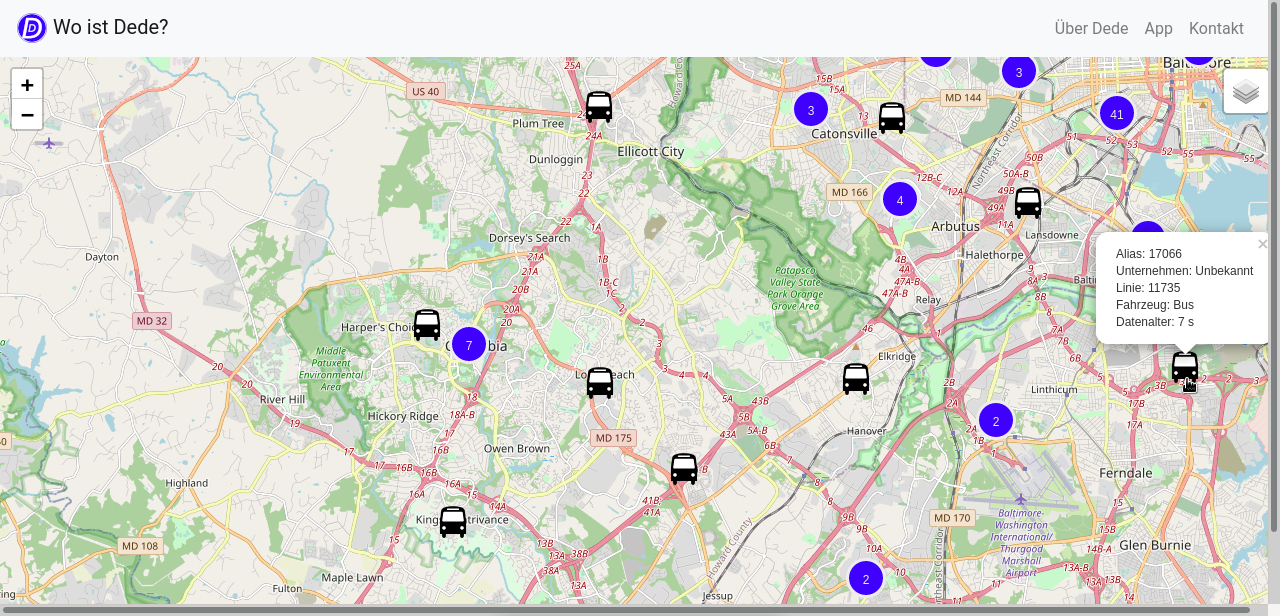
\includegraphics[width=\paperwidth]{dede/dede_real-time_map_crop}};
}

\begin{frame}{Dede Konzept}
  %alternative alignment to center is left and right
  \begin{center}
    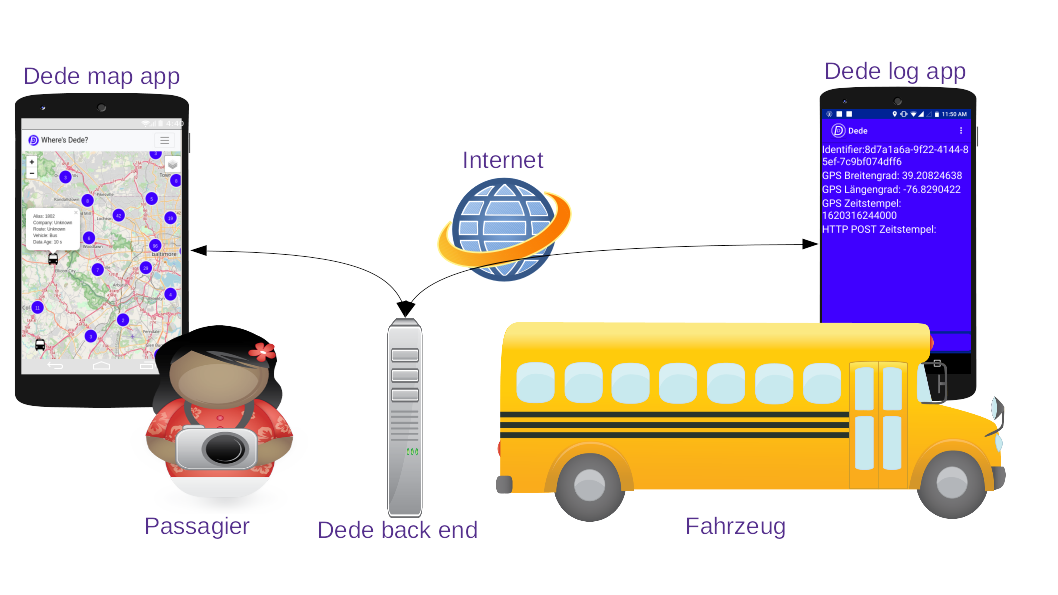
\includegraphics[width=\paperwidth]{dede/dede-concept}
  \end{center}
\end{frame}

\begin{frame}{Dede Konzept}
  Die Dede Echtzeit-Karte besteht aus drei Komponenten:
  \begin{itemize}
  \item Die Dede-App für Smartphones zeichnet die Bewegungsdaten des Fahrzeugs auf und überträgt sie per Internet an den Dede-Server.
  \item Der Dede-Server vermittelt zwischen Dede-App und Dede-Karte, so das die Karte NICHT jede App separat abfragen muss.
  \item Die Dede-Karte visualisiert die Bewegungdaten auf einer Karte in Echtzeit.
  \end{itemize}
\end{frame}

\egroup
